% !TeX root = probability.tex

%%%%%%%%%%%%%%%%%%%%%%%%%%%%%%%%%%%%%%%%%%%%%%%%%%%%%%%%%%%%%

%%%%%%%%%%%%%%%%%%%%%%%%%%%%%%%%%%%%%%%%%%%%%%%%%%%%%%%%%%%%%%

\section{קיץ תשע"ה מועד ב}

\begin{center}
\selectlanguage{english}
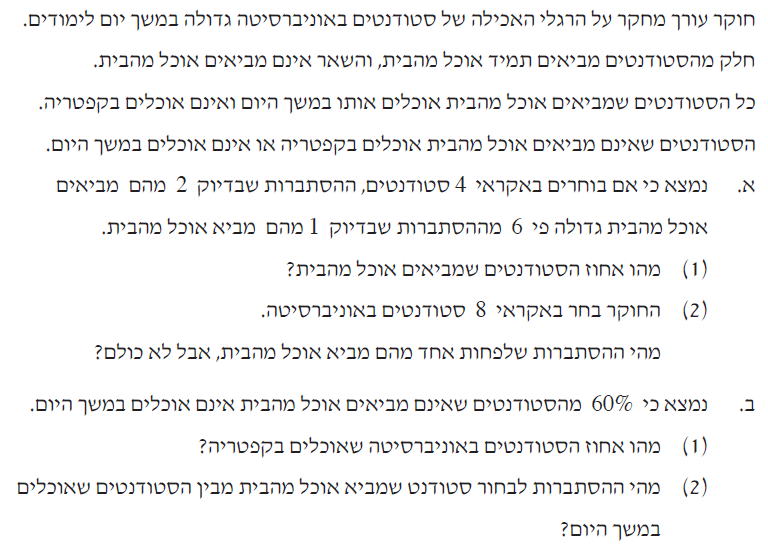
\includegraphics[width=.85\textwidth]{summer-2015b-3}
\end{center}

\textbf{סעיף א (1)}

נסמן את המאורע "מביא אוכל מהבית" ב-%
$M$ \L{mavi}
ונסמן
$b=P(M)$.
המילה "בדיוק" מכוון לנוסחת ברנולי:
\begin{eqn}
{4 \choose 2} b^2(1-b)^2 &=& 6\cdot {4 \choose 1} b (1-b)^3\\
6b&=&24(1-b)\\
b&=&\frac{4}{5}\,.
\end{eqn}
השאלה שואלת על "אחוז" ולכן התשובה היא
$80\%$.

\textbf{סעיף א (2)}

ההסתברות של "לפחות אחד אבל לא כולם" היא המשלים ל-"לא אפס ולא כולם":
\[
1-\left(\frac{1}{5}\right)^8-\left(\frac{4}{5}\right)^8=0.8322\,.
\]

\textbf{סעיף ב (1)}

נסמן את המאורע "אוכל בקפטריה" ב-%
$C$ \L{(cafeteria)}.
בעץ ההסתברויות בעמוד הבא הכוכבית מראה את מהמסלול עבור המאורע 
$C$
ולכן:
\[
P(C)=\frac{1}{5}\cdot \frac{4}{10} = \frac{2}{25}\,.
\]

\begin{figure}
\begin{center}
\begin{tikzpicture}
[grow=right,
level 1/.append style={level distance=3cm,sibling distance=6em},
level 2/.append style={text width=1cm,level distance=4cm,sibling distance=8em}]
\node[text width=1cm] {} % root
child {
  node {}
    edge from parent node[below,xshift=-5mm,yshift=-3mm] {\R{מביא מהבית}}
      node[above,xshift=3mm,yshift=-4pt] {$\frac{4}{5}$}
}
child { 
  node {}
    child {
      node {$*$}
      edge from parent node[below,xshift=5mm,yshift=-3mm] {\R{אוכל בקפטריה}}
        node[above,xshift=11mm,yshift=-2mm] {$\frac{4}{10}$}
    }
    child {
      node {}
      edge from parent node[above,xshift=5mm,yshift=3mm] {\R{לא אוכל}}
        node[below,xshift=10mm,yshift=2mm] {$\frac{6}{10}$}
    }
    edge from parent node[above,xshift=-4mm,yshift=5mm] {\R{לא מביא מהבית}}
      node[below,xshift=4mm,yshift=2mm] {$\frac{1}{5}$}
};
\end{tikzpicture}
\end{center}
\end{figure}
פתרון זה לא כל כך מוצא חן בעיני כי לא ברור מאיפה צץ העץ שבדרך כלל משמש למאורעות סדרתיות כגון הטלת קוביות מספר פעמים. אני מעדיף פתרון מבוסס הסתברות מותנית ואני חושב שניסוח השאלה היתה צריכה להיות "%
\textbf{מבין}
אלה שלא מביאים אוכל
$60\%$
אינם אוכלים בקפטריה". לפי נוסחת ההסתברות השלמה:
\[
P(C) = P(C/M)P(M) + P(C/\overline{M})P(\overline{M})=
0\cdot 0.8 + (1-0.6)\cdot (1-0.8)=0.4\cdot 0.2=0.08\,.
\]


\textbf{סעיף ב (2)}

נסמן ב-%
$O$ \L{(okhel)}
את המאורע "מביא אוכל. המילה
"\textbf{מבין}"
מכוונת להסתברות מותנית, ונחשב אותה תוך שימוש בעובדה ש-%
$M\subseteq O$
ןלכן
$M\cap O = M$:
\begin{eqn}
P(M/O) &=& \frac{P(M \:\cap\: O)}{P(O)}\\
&=& \frac{P(M)}{P(O)}\\
&=&\frac{\frac{4}{5}}{\frac{4}{5}+\frac{2}{25}}=\frac{10}{11}\,.
\end{eqn}

%%%%%%%%%%%%%%%%%%%%%%%%%%%%%%%%%%%%%%%%%%%%%%%%%%%%%%%%%%%%%

\section{קיץ תשע"ה מועד א}

\begin{center}
\selectlanguage{english}
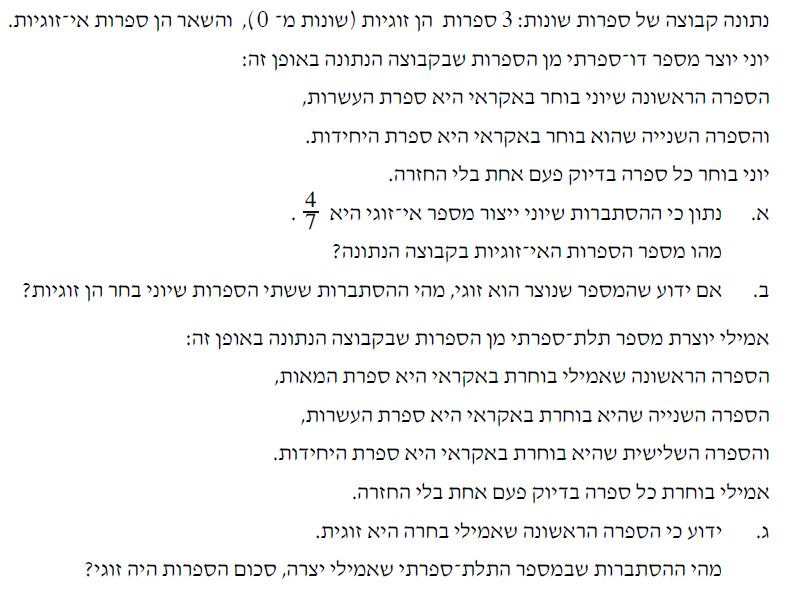
\includegraphics[width=.9\textwidth]{summer-2015a-3}
\end{center}

\textbf{סעיף א}

נסמן את קבוצת הספרות ב-%
$S$ \L{(sifarot)},
קבוצת הספרות הזוגיות ב-%
$Z$ \L{(zugi)},
קבוצת הספרות האי-זוגיות ב-%
$I$ \L{(i-zugi)}.
בחירה של ספרת העשרות ואחר כך ספרת היחידות מכוונת לעץ הסתברויות. במקום לרשום את מספרי הספרות בצמתים וההסתברויות על הקשתות, נפשט את התרשים ונרשום בכל צומת את ההסתברויות שליפת ספרה זוגית או אי-זוגית
$(P(Z=k_1),P(I=k_2))$.

\begin{center}
\begin{tikzpicture}
[grow=right,
level 1/.append style={text width=2cm,level distance=3.5cm,sibling distance=6em},
level 2/.append style={text width=2.5cm,level distance=4.5cm,sibling distance=3.5em}]
\node[text width=2cm] {$\left(\frac{3}{n},\frac{n-3}{n}\right)$} % root
child {
  node {$\left(\frac{3}{n-1},\frac{n-4}{n-1}\right)$}
    child {
      node {$\left(\frac{3}{n-2},\frac{n-5}{n-2}\right)\quad *$}
      edge from parent node[below,xshift=5mm,yshift=-1mm] {\R{אי-זוגי}}
    }
    child {
      node {$\left(\frac{2}{n-2},\frac{n-4}{n-2}\right)$}
      edge from parent node[above,xshift=5mm,yshift=1mm] {\R{זוגי}}
    }
    edge from parent node[below,yshift=-1mm] {\R{אי-זוגי}}
}
child { 
  node {$\left(\frac{2}{n-1},\frac{n-3}{n-1}\right)$}
    child {
      node {$\left(\frac{2}{n-2},\frac{n-4}{n-2}\right)\quad *$}
      edge from parent node[below,xshift=5mm,yshift=-1mm] {\R{אי-זוגי}}
    }
    child {
      node {$\left(\frac{1}{n-2},\frac{n-3}{n-2}\right)$}
      edge from parent node[above,xshift=5mm,yshift=1mm] {\R{זוגי}}
    }
    edge from parent node[above] {\R{זוגי}}
};
\end{tikzpicture}
\end{center}
המאורע
$YI$
שיוני ייצור מספר אי-זוגי יתרחש רק אם הבחירתו השנייה היא ספרה אי-זוגית. המסלולים המתאימים מסומנים בתרשים בכוכביות. נחשב את ההסתברות ונשווה להסתברות הנתונה:
\begin{eqn}
P(YI)&=&\frac{3}{n}\cdot\frac{n-3}{n-1} \;+\; \frac{n-3}{n}\cdot\frac{n-4}{n-1} = \frac{4}{7}\\
4n(n-1)&=&7(n-3)(n-1)\\
n&=&7\\
|I|&=&n-3=4\,.
\end{eqn}
נתון ש-%
$n\geq 3$
ולכן
$n\neq 1$
וניתן לצמצם את 
$n-1$.

\textbf{סעיף ב}

במספר זוגי הספרה האחרונה זוגית. נסמן ב-%
$Z2$
את המאורע ששתי הספרות זוגיות ונסמן ב-%
$ZA$ \L{aharona}
את המאורע ספרה אחרונה זוגית. הניסוח
"\textbf{אם ידוע}"
מכוון להסתברות מותנית:
\begin{eqn}
P(Z2/ZA) &=& \frac{P(Z2\:\cap\:ZA)}{P(ZA)}\\
&=&\frac{P(Z2)}{P(ZA)}\\
&=&\frac{\frac{3}{7}\cdot\frac{2}{6}}{1-\frac{4}{7}}=\frac{1}{3}\,.
\end{eqn}
השתמשנו ב-%
$Z2\subseteq ZA$ 
כי אם שתי הספרות זוגיות אזי הספרה האחרונה זוגית, ובעובדה ש-%
$P(ZA)=1-P(YI)$
שחישבנו בסעיף הקודם. החישוב של
$P(Z2)$
היא ההסתברות שמתקבלת מהמסלול העליון בעץ עבור בחירה של שתי ספרות זוגיות.

\textbf{סעיף ג}

הסכום יהיה זוגי רק אם שתי הספרות האחרונת הן זוגיות או אי-זוגיות:
\begin{eqn}
2k_1+2k_2+2k_3&=&2(k_1+k_2+k_3)\\
2k_1+2(k_2+1)+2(k_3+1)&=&2(k_1+k_2+k_3+1)\,.
\end{eqn}
נסמן ב-%
$Z1$
את המאורע שהספרה הראשונה זוגית ונסמן ב-%
$S$ \L{(sekhum)}
את המאורע שסכום הספרות זוגי. המילה "ידוע" מכוון להסתברות מותנית ולכן:
\begin{eqn}
P(S/Z1)&=& \frac{P(S\:\cap\:Z1)}{P(Z1)}\\
&=& \frac{P(S\:\cap\:Z1)}{P(Z1)}\\
&=&\frac{\frac{3}{7}\cdot\frac{2}{6}\cdot \frac{1}{5}+
\frac{3}{7}\cdot\frac{4}{6}\cdot \frac{3}{5}}
{\frac{3}{7}}=\frac{7}{15}\,.
\end{eqn}
המנה חושב משני המסלולים המסומנים בכוכביות בעץ ההסתברויות בעמוד הבא, כי הם מתחילים עם בחירה של ספרה זוגית ואז שני ואז או שתי ספרות זוגיות או שתי ספרות אי-זוגיות כדי לקבל סכום זוגי.
\begin{center}
\begin{tikzpicture}
[grow=right,
level 1/.append style={level distance=3cm,sibling distance=10em},
level 2/.append style={level distance=3cm,sibling distance=10em},
level 3/.append style={level distance=4cm,sibling distance=5em}]
\node {$\left(\frac{3}{7},\frac{4}{7}\right)$} % root
  child {
    node {$\cdots$}
    edge from parent node[below,yshift=-8pt] {\R{אי-זוגי}}
  }
child {
  node {$\left(\frac{2}{6},\frac{4}{6}\right)$}
child {
  node {$\left(\frac{2}{5},\frac{3}{5}\right)$}
    child {
      node {$\left(\frac{2}{4},\frac{2}{4}\right)\quad *$}
      edge from parent node[below,xshift=5mm,yshift=-2mm] {\R{אי-זוגי}}
    }
    child {
      node {$\left(\frac{1}{4},\frac{3}{4}\right)$}
      edge from parent node[above,xshift=5mm,yshift=2mm] {\R{זוגי}}
    }
    edge from parent node[below,yshift=-3mm] {\R{אי-זוגי}}
}
child { 
  node {$\left(\frac{1}{5},\frac{4}{5}\right)$}
    child {
      node {$\left(\frac{1}{4},\frac{3}{4}\right)$}
      edge from parent node[below,xshift=5mm,yshift=-2mm] {\R{אי-זוגי}}
    }
    child {
      node {$\left(\frac{0}{4},\frac{4}{4}\right)\quad *$}
      edge from parent node[above,xshift=5mm,yshift=2mm] {\R{זוגי}}
    }
    edge from parent node[above,yshift=2mm] {\R{זוגי}}
}
  edge from parent node [above,yshift=8pt] {\R{זוגי}}
};
\end{tikzpicture}
\end{center}

%%%%%%%%%%%%%%%%%%%%%%%%%%%%%%%%%%%%%%%%%%%%%%%%%%%%%%%%%

\newpage

\section{חורף תשע"ה}

\begin{center}
\selectlanguage{english}
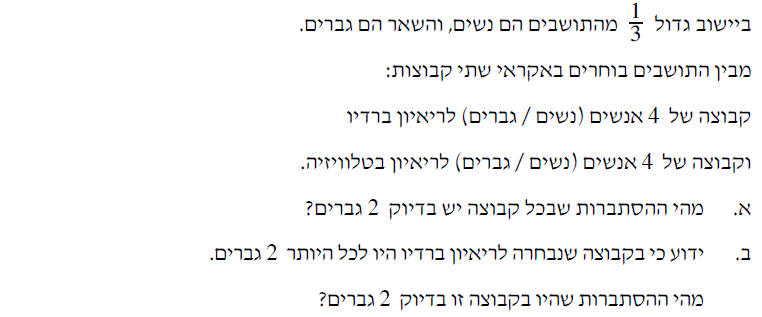
\includegraphics[width=.85\textwidth]{winter-2015-3}
\end{center}

המשמעות של "יישוב גדול" היא (כנראה) שאפשר לבחור את שתי הקבוצות בלי לשנות את ההסתברות של 
$\frac{1}{3}$
במהלך הבחירה, למרות שהבחירה היא ללא החזרה.

\textbf{סעיף א}

נסמן ב-%
$G2$
את המאורע של בחירת שני בגברים בקבוצה אחת ונסמן ב-%
$G22$
את המאורע של בחירת שני גברים בשתי הקבוצות. בחירת גבר נקראת הצלחה ולכן נשתמש בנוסחת ברנולי כדי לקבל את ההסתברות
\textbf{לבדיוק}
שתי הצלחות בקבוצה אחת:
\[
P(G2)={4 \choose 2}\left(\frac{2}{3}\right)^2\left(1-\frac{2}{3}\right)^2=\frac{8}{27}\,.
\]
לפי ההנחה שאין שינוי בהסתברות של הבחירה בין שתי הקבוצות, נקבל:
\[
P(G22)=P(G2)\cdot P(G2)=\frac{64}{729}\,.
\]

\textbf{סעיף ב}

נסמן את המאורע "לכל היותר שני גברים" ב-%
$G012$.
הניסוח
"\textbf{ידוע כי}"
מכוון להסתברות מותנית:
\begin{eqn}
P(G2/G012)&=&\frac{P(G2 \:\cap\: G012)}{P(G012)}\\
\end{eqn}
$G2\subseteq G012$
ולכן המנה היא
$G2=\frac{8}{27}$.
"לכל היותר שני גברים" הוא הסכום של שלוש נוסחאות ברנולי:
\[
\left(\frac{2}{3}\right)^0\left(\frac{1}{3}\right)^4 + {4\choose 1}\left(\frac{2}{3}\right)^1\left(\frac{1}{3}\right)^3 + {4\choose 2}\left(\frac{2}{3}\right)^2\left(\frac{1}{3}\right)^2=\frac{11}{27}\,
\]
והתשובה לשאלה היא:
\[
P(G2/G012)=\frac{\frac{8}{27}}{\frac{11}{27}}=\frac{8}{11}\,.
\]

